%%%%%%%%%%%%%%%%%%%%%%%%%%%%%%%%%%%%%%%%%%%%%%%%%%%%%%%%%%%%%%%%%%%%
%% I, the copyright holder of this work, release this work into the
%% public domain. This applies worldwide. In some countries this may
%% not be legally possible; if so: I grant anyone the right to use
%% this work for any purpose, without any conditions, unless such
%% conditions are required by law.
%%%%%%%%%%%%%%%%%%%%%%%%%%%%%%%%%%%%%%%%%%%%%%%%%%%%%%%%%%%%%%%%%%%%

\documentclass{beamer}
\usetheme[faculty=fi]{fibeamer}
\usepackage[utf8]{inputenc}

\usepackage[
  main=czech, %% By using `czech` or `slovak` as the main locale
                %% instead of `english`, you can typeset the
                %% presentation in either Czech or Slovak,
                %% respectively.
  english, slovak %% The additional keys allow foreign texts to be
]{babel}        %% typeset as follows:
%%
%%   \begin{otherlanguage}{czech}   ... \end{otherlanguage}
%%   \begin{otherlanguage}{slovak}  ... \end{otherlanguage}
%%
%% These macros specify information about the presentation
\title{Používání a získávání kryptoměny Monero z pohledu použitelné bezpečnosti} %% that will be typeset on the

\subtitle{21. června 2019} %% title page.
\author{Bc. Radim Lipovčan, 433279@muni.cz}
%% These additional packages are used within the document:
\usepackage{ragged2e}  % `\justifying` text
\usepackage{booktabs}  % Tables
\usepackage{tabularx}
\usepackage{tikz}      % Diagrams
\usetikzlibrary{calc, shapes, backgrounds}
\usepackage{amsmath, amssymb}
\usepackage{url}       % `\url`s
\usepackage{listings}  % Code listings
\frenchspacing

\usepackage{graphicx}
\graphicspath{ {./resources/} }
\usepackage{multicol}
\begin{document}

  \frame{\maketitle}

  \AtBeginSection[]{% Print an outline at the beginning of sections
    \begin{frame}<beamer>
      \frametitle{Obsah sekce \thesection}
		\begin{multicols}{2}      
      \tableofcontents[currentsection]
      \end{multicols}
    \end{frame}}

  \begin{darkframes}
    \section{Motivace}
    \subsection{SSME}
    \begin{frame}{Motivace | SSME}
    Při výběru tématu bylo potřeba dbát pozor na:
		\begin{itemize}
		\item Důraz na T-shape, jak jej zohlednit v diplomové práci?
		\item "Diplomová práce by měla reflektovat tvůj Interim Projekt nebo alespoň zkušenosti v něm nabyté." \begin{itemize}
		\item převzato z http://ssme.fi.muni.cz/student/studium)
		\end{itemize}
		\end{itemize}		     
     
	    \end{frame}
    \subsection{Monero}
    \begin{frame}{Motivace | Monero}
		\begin{itemize}
		\item Open-source kryptoměna
    	\item Zaměření na anonymitu, decentralizaci
     	\item Aktivní komunita na GitHubu a na Redditu včetně dalších sociálních sítí
		\end{itemize}  
		\begin{figure}
  \centering
  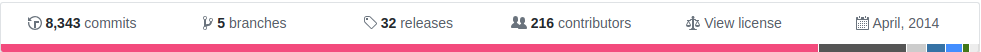
\includegraphics[width=1\textwidth]{monero-github.png}
  
\includegraphics[width=0.4\textwidth]{monero-reddit.png}
  \caption{Monero Github \& Reddit.}  \label{fig:xray}
\end{figure}
		  
    \end{frame}
    \subsection{Cíl diplomové práce}
    \begin{frame}{Motivace | Cíl diplomové práce}
     Zkombinovat:
     \begin{itemize}
     \item Znalosti nabyté na intermu, studiu, rozsah T-shape
     \item Technické téma kryptoměny Monero
     \end{itemize}
     	Cílem:
		\begin{itemize}
		\item Zmapovat způsoby získávání a užívání kryptoměny Monero
		\item Uživatelská část - využití kryptoměny
		\item Těžební část - software, pooly, systémy pro těžbu
		\item Obě části - provést výzkum na dané části komunity
		\begin{itemize}
		\item A vytěžit z toho nové věci - best practices + automatizace
		\end{itemize}
		\end{itemize}
    \end{frame}
  \end{darkframes}

  \AtBeginSection[]{% Print an outline at the beginning of sections
    \begin{frame}<beamer>
      \frametitle{Obsah sekce \thesection}
      \begin{multicols}{2}      
      \tableofcontents[currentsection]
      \end{multicols}
    \end{frame}}
    
  \begin{darkframes}
    \section{Kryptoměna Monero}
    \subsection{Informace o krypoměně}
    \begin{frame}{Kryptoměna Monero | Informace o krypoměně}
    Open-source kryptoměna vyvíjená pod Monero projektem.
    Cílem je mít decentralizovanou a anonymní kryptoměnu.
    
\begin{itemize}[<+->]
\item<1-4>  Žádnou transakci nelze jednoduše vysledovat zpátky k uživateli a ani nelze zjistit kolik Monera bylo posláno.
\item<2-4> Použití CryptoNote protokolu.
\item<3-4> Blockchain je veřejný, většina je šifrovaná.
\item<4-4> Pro anonymitu krpytoměny jsou použity technologie: 
\begin{itemize}
\item Ring Signatures (skrytí odesílatele)
\item RingCT (skrytí posílané částky)
\item Stealth Addresses (skrytí příjemce a historie transakce)
\end{itemize}
\end{itemize}    

     \begin{figure}
  
\includegraphics[width=0.2\textwidth]{monero-icon.png}
  \caption{Monero Github \& Reddit.}  \label{fig:xray}
\end{figure}
    \end{frame}
    \subsection{Popis systému}
    \begin{frame}{Kryptoměna Monero | Popis systému}
   Před samotným výzkumem a tvorbou:
     \begin{itemize}[<+->]
     \item<1-3> Vývojový cyklus
     \item<1-3> Princip transakcí
     \item<2-3> Fungování peněženek
     \item<2-3> Útoky vůči peněženkám
     \item<3-3> Problémy Monera (většinou malware)
     \end{itemize}
    \end{frame}
  \end{darkframes}


  \AtBeginSection[]{% Print an outline at the beginning of sections
    \begin{frame}<beamer>
      \frametitle{Obsah sekce \thesection}
      \begin{multicols}{2}      
      \tableofcontents[currentsection]
      \end{multicols}
    \end{frame}}
    
   
  \begin{darkframes}
    \section{Výzkum uživatelů Monera}
    \subsection{Cíl}
    \begin{frame}{Cíl výzkumu uživatelů Monera}
Zjistit informace o chování uživatelů při používání Monera a zároveň se zaměřit na práci s klíči k peněžence včetně zaměření se na samotnou bezpečnost užívání.

Dotazník rozdělen:
\begin{itemize}
\item<1-4> G01 - Introductory information
\item<1-4> G02 - Monero usage
\item<2-4> G03 - Monero key and coin management
\item<3-4> G04 - Monero and malicious things
\item<4-4> G05 - Monero recovery
\item<4-4> G06 - Special question set for miners
\item<4-4> G07 - Demographics
	\end{itemize}
	\end{frame}
    \subsection{Sběr dat}
    \begin{frame}{Sběr dat}
     \begin{itmeize}
     \item 15.11.2018 - 27.01.2019
     \item LimeSurvey, na vlastním serveru
     \item Respondentům bylo doporučeno použít TOR nebo alespoň proxy
     \item CAPTCHA proti spamu a botům
     \end{itemize}
    \end{frame}
    \subsection{Výsledky}
    \begin{frame}{Výsledky}
     Obsah
    \end{frame}
    \subsection{Nejlepší praktiky}
    \begin{frame}{Nejlepší praktiky}
     Obsah
    \end{frame}
  \end{darkframes}
  
  \AtBeginSection[]{% Print an outline at the beginning of sections
    \begin{frame}<beamer>
      \frametitle{Obsah sekce \thesection}
      \begin{multicols}{2}      
      \tableofcontents[currentsection]
      \end{multicols}
    \end{frame}}
    
  \begin{darkframes}
    \section{Výzkum těžařů Monera}
    \subsection{Cíl}
    \begin{frame}{Cíl výzkumu těžařů Monera}
     Obsah
    \end{frame}
    \subsection{Sběr dat}
    \begin{frame}{Sběr dat}
     Obsah
    \end{frame}
    \subsection{Nasbíraná data}
    \begin{frame}{Nasbíraná data}
     Obsah
    \end{frame}
    \subsection{Výsledky}
    \begin{frame}{Výsledky}
     Obsah
    \end{frame}
    \subsection{Automatizace}
    \begin{frame}{Automatizace}
     Obsah
    \end{frame}
  \end{darkframes}
  
  \AtBeginSection[]{% Print an outline at the beginning of sections
    \begin{frame}<beamer>
      \frametitle{Obsah sekce \thesection}
      \begin{multicols}{2}      
      \tableofcontents[currentsection]
      \end{multicols}
    \end{frame}}
    
  \begin{darkframes}
    \section{Závěr}
    \subsection{Webový portál}
    \begin{frame}{Webový portál}
     Obsah
    \end{frame}
    \subsection{Open-source}
    \begin{frame}{Open-source}
     Obsah
    \end{frame}
  \end{darkframes}
  
  \begin{frame}{}
\end{frame}
    
  \AtBeginSection[]{% Print an outline at the beginning of sections
    \begin{frame}<beamer>
      \frametitle{Obsah sekce \thesection}
      \begin{multicols}{2}      
      \tableofcontents[currentsection]
      \end{multicols}
    \end{frame}}
    
  \begin{darkframes}
    \section{Reakce na posudky, dotazy}
    \subsection{Název sekce}
    \begin{frame}{Název frame}
     Obsah
    \end{frame}
  \end{darkframes}

\end{document}
